\chapter{Results and Discussion}\label{ch5:chapter5}


\section{Experiments results Database }\label{ch5:database}

The main objective of this study was to propose an evaluation of three failure criteria for a selected rock, Dunnville Sandstone. As explained in the previous chapters, their empirical nature requires a thick database of diverse multi axial experiments for their development. 

Dunnville Sandstone have been used for several works in the past and particularly for multi axial experiments \cite{Labuz2018}\cite{Zeng2019}\cite{Tarokh2016}. The ones performed in the scope of this study (cf. Chapter \ref{ch4:title}) presented the opportunity to enrich the existing tests results database and to evaluate the failure criteria with data representative of Dunnville Sandstone response.

The database presented in Table \ref{tb5:database} was based on the one proposed by Zeng et al. (2019) \cite{Zeng2019}, and extended with the results of the experiments from this study. In this table, each experiment is associated with the following elements: the orientation of the bedding regarding the application of the axial stress, the three principal stresses (i.e. $\sigma_I$,$\sigma_{II}$,$\sigma_{III}$) and the stress invariants (i.e.$p$, $q$, $\theta$)

This database was used for the evaluation of Mohr-Coulomb,Hoek-Brown and Paul-Mohr-Coulomb failure criteria, that will be presented in the following sections.

\begin{table}
    \centering
    \begin{tabular}{cccccccc}
        \hline 
        Test & Bedding & $\sigma_I$ [\si{MPA}] & $\sigma_{II}$ [\si{MPA}] &$\sigma_{III}$ [\si{MPA}] & $p$ [\si{MPA}] & $q$ [\si{MPA}] & $\theta$ [\si{\degree}] \\
        \hline
        \hline
        Published TC-1 & \(\perp\) & 29.7 & 0.0 & 0.0 & 9.9 & 29.7 & 0 \\
        Published TC-2 & \(\perp\) & 39.4 & 2.5 & 2.5 & 14.8 & 36.9 & 0 \\
        Published TC-3 & \(\perp\) & 52.9 & 5.0 & 5.0 & 21.0 & 47.9 & 0 \\
        Published TC-4 & \(\perp\) & 71.5 & 10.0 & 10.0 & 30.5 & 61.5 & 0 \\
        Published TC-5 & \(\perp\) & 98.4 & 20.0 & 20.0 & 46.1 & 78.4 & 0 \\
        Published TC-6 & \(\perp\) & 114.5 & 30.0 & 30.0 & 58.2 & 84.5 & 0 \\
        Published TC-7 & \(\perp\)& 129.4 & 40.0 & 40.0 & 69.8 & 89.4 & 0 \\
        Published TC-8 & \(\perp\) & 142.1 & 50.0 & 50.0 & 80.7 & 92.1 & 0 \\
        Published TC-9 & \(\perp\) & 153.8 & 60.0 & 60.0 & 91.3 & 93.8 & 0 \\
        Published TC-10 & \(\|\) & 24.9 & 0.0 & 0.0 & 8.3 & 24.9 & 0 \\
        Published TC-11 & \(\|\) & 35.2 & 2.5 & 2.5 & 13.4 & 32.7 & 0 \\
        Published TC-12 & \(\|\) & 48.8 & 5.0 & 5.0 & 19.6 & 43.8 & 0 \\
        Published TC-13 & \(\|\) & 68.0 & 10.0 & 10.0 & 29.3 & 58.0 & 0 \\
        Published TC-14 & \(\|\) & 95.9 & 20.0 & 20.0 & 45.3 & 75.9 & 0 \\
        Published TC-15 & \(\|\) & 110.9 & 30.0 & 30.0 & 57.0 & 80.9 & 0 \\
        Published TC-16 & \(\|\) & 125.5 & 40.0 & 40.0 & 68.5 & 85.5 & 0 \\
        Published TC-17 & \(\|\) & 138.1 & 50.0 & 50.0 & 79.4 & 88.1 & 0 \\
        Published TC-18 & \(\|\) & 150.8 & 60.0 & 60.0 & 90.3 & 90.8 & 0 \\
        UCS   & \(\perp\) & 29.8 & 0 & 0   & 27.95 & 51.43 & 0 \\ 
        TC 9  & \(\perp\) & 49.43 & 5  & 5 & 19.81 & 44.43 & 0 \\ 
        TC 0  & \(\perp\) & 61.43 & 10 & 10 & 27.95 & 51.43 & 0 \\ 
        TC 5  & \(\perp\) & 91.08 & 20 & 20 & 44.72 & 71.08 & 0 \\ 
        TC 8  & \(\perp\) & 127.3 & 40 & 40 & 65.73 & 87.30 & 0 \\ 
        TC 10 & \(\perp\) & 151.1 & 60 & 60 & 88.12 & 91.10 & 0 \\ 
        \hline
        \hline
        Published TE-1 & \(\perp\) & 35.0 & 35.0 & 0.8 & 23.6 & 34.2 & 60 \\
        Published TE-2 & \(\perp\) & 40.0 & 40.0 & 1.2 & 27.1 & 38.8 & 60 \\
        Published TE-3 & \(\perp\) & 50.0 & 50.0 & 6.0 & 35.3 & 44.0 & 60 \\
        Published TE-4 & \(\perp\) & 60.0 & 60.0 & 10.1 & 43.4 & 49.9 & 60 \\
        Published TE-5 & \(\perp\) & 69.0 & 69.0 & 11.5 & 49.8 & 57.5 & 60 \\
        Published TE-6 & \(\|\) & 40.0 & 40.0 & 1.8 & 27.3 & 38.2 & 60 \\
        Published TE-7 & \(\|\) & 50.0 & 50.0 & 5.7 & 35.2 & 44.3 & 60 \\
        Published TE-8 & \(\|\) & 60.0 & 60.0 & 8.0 & 42.7 & 52.0 & 60 \\
        TE 3  & \(\perp\) & 35 & 35 & 3.96 & 24.64 & 31.08 & 60 \\ 
        TE 1  & \(\perp\) & 40 & 40 & 4.50 & 27.89 & 36.34 & 60 \\ 
        TE 2  & \(\perp\) & 60 & 60 & 9.68 & 43.01 & 50.98 & 60 \\
        \hline
        \hline
        Published TT-1 & \(\perp\) & 48.3 & 31.6 & 5.0 & 28.3 & 37.8 & 37.5 \\
        Published TT-2 & \(\perp\) & 52.9 & 25.1 & 7.0 & 28.3 & 40.1 & 22.7 \\
        Published TT-3 & \(\perp\) & 63.9 & 12.1 & 9.0 & 28.3 & 53.4 & 2.9 \\
        Published TT-4 & \(\perp\) & 70.6 & 49.4 & 15.0 & 45.0 & 48.7 & 37.8 \\
        Published TT-5 & \(\perp\) & 77.5 & 70.5 & 20.0 & 56.0 & 54.3 & 53.5 \\
        Published TT-6 & \(\perp\) & 83.9 & 62.1 & 22.0 & 56.0 & 54.4 & 39.7 \\
        TT 1 & \(\perp\) & 88.14 & 46.85 & 10 & 48.33 & 55.28 & 28.12 \\
        TT 2 & \(\perp\) & 99.98 & 20 & 20 & 46.65 & 62.28 & 0 \\
        \hline
    \end{tabular}
    \caption{Database of experiments results for Dunnville Sandstone. The "Published" data are from Zeng et al. \cite{Zeng2019}}
    \label{tb5:database}
\end{table}

\section{Evaluation of the failure criteria}\label{ch5:evaluation}

The Mohr-Coulomb, Hoek-Brown and Paul-Mohr-Coulomb failure criteria presented in Chapter \ref{ch2:title} were fitted to the experiment results from Table \ref{tb5:database}. A computation program was developed for the fittings using the programming language Python. All the resources needed to access the program files are listed in Appendix REF{APPENDIX B}. 

\subsection{Mohr-Coulomb failure criterion}

The Mohr-Coulomb failure criterion is formulated in terms two principal stresses (cf. Equations \ref{eq2:MCfinalform} and \ref{eq2:MCcondenseform}) and unique strength parameters (i.e. $\phi$,$c$), therefore, the parameters fitting was done using only axisymmetric triaxial compression tests results (i.e. $\theta = 0^\circ$). 

From this fitting, the coefficient $K_p$ was determined and the other parameters were computed: 
\begin{equation}
    K_p = 2.55 \quad \textrm{and} \quad C_0 = 29.7
\end{equation}
\begin{equation}
    \phi = \frac{K_p-1}{K_p+1} = 25.9^\circ
\end{equation}
\begin{equation}
    c = \frac{C_0(1-sin\phi)}{2cos\phi} = 9.30
\end{equation}
\begin{equation}
    V_0 = \frac{C_0}{K_p-1} = 19.2
\end{equation}

Knowing the strength parameters, the Mohr-Coulomb failure surface is plotted in the $(\sigma_3-\sigma_1)$ plane using Equation \ref{eq2:MCfinalform}(cf. Figure \ref{fig5:mc_sig1sig3}).

\begin{figure}[tb]
    \centering
    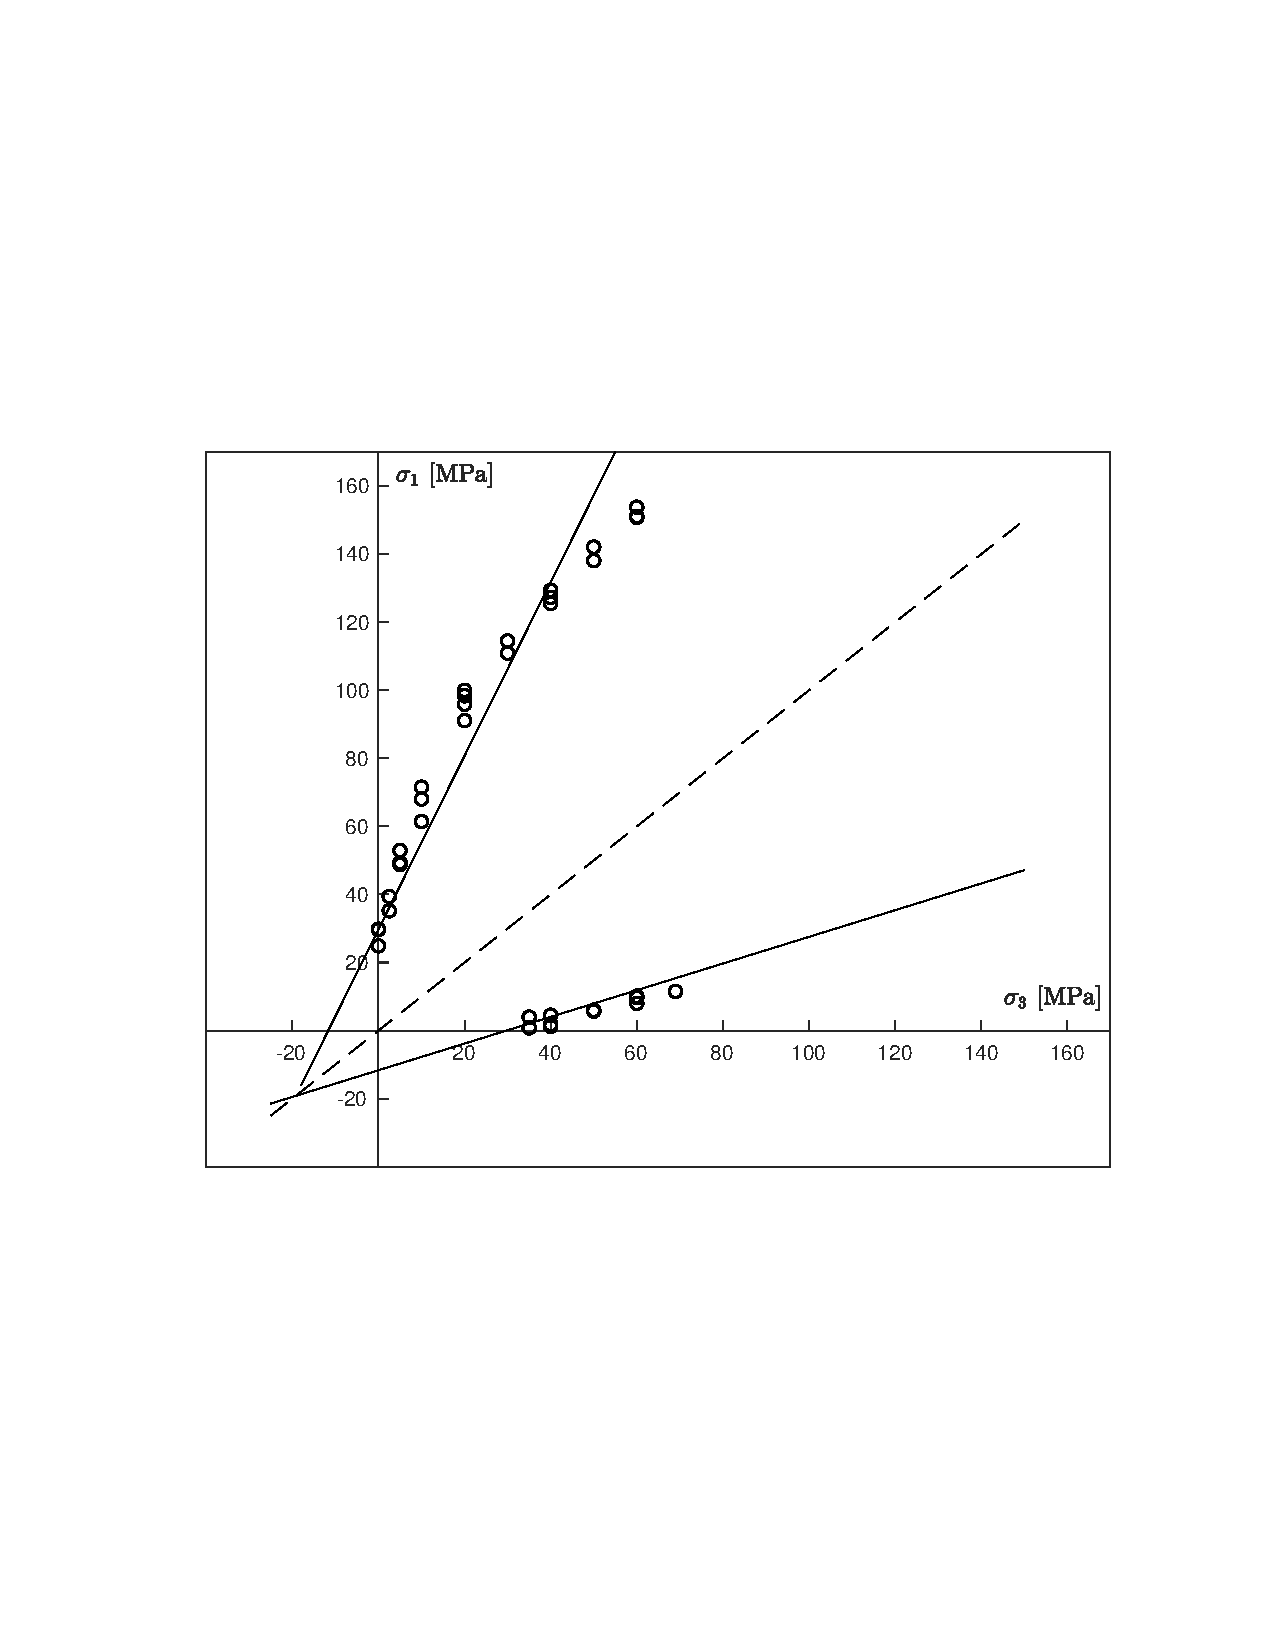
\includegraphics[width=\columnwidth]{ch5/mc_sig1sig3}
    \caption{Mohr-Coulomb criterion failure surface in  $(\sigma_3-\sigma_1)$ plane}
    \label{fig5:mc_sig1sig3}
\end{figure} 

The criterion was also fitted in the $(p-q)$ plane, for which the plot obtained is shown in Figure \ref{fig5:mc_pq}. The coefficients $m_{c,e}$ and $b_{c,e}$ were computed using Equations \ref{eq2:MC_mc_q} to \ref{eq2:MC_be_q}:

\begin{equation}
    m_c = \frac{6 \sin \phi}{3-\sin \phi} = 1.02
\end{equation}
\begin{equation}
    m_e = \frac{6 \sin \phi}{3+\sin \phi} = 0.76
\end{equation}
\begin{equation}
    b_c = \frac{6 c \cos \phi}{3-\sin \phi} = 19.6
\end{equation}
\begin{equation}
    b_e = \frac{6 c \cos \phi}{3+\sin \phi} = 14.6
\end{equation}


\begin{figure}[tb]
    \centering
    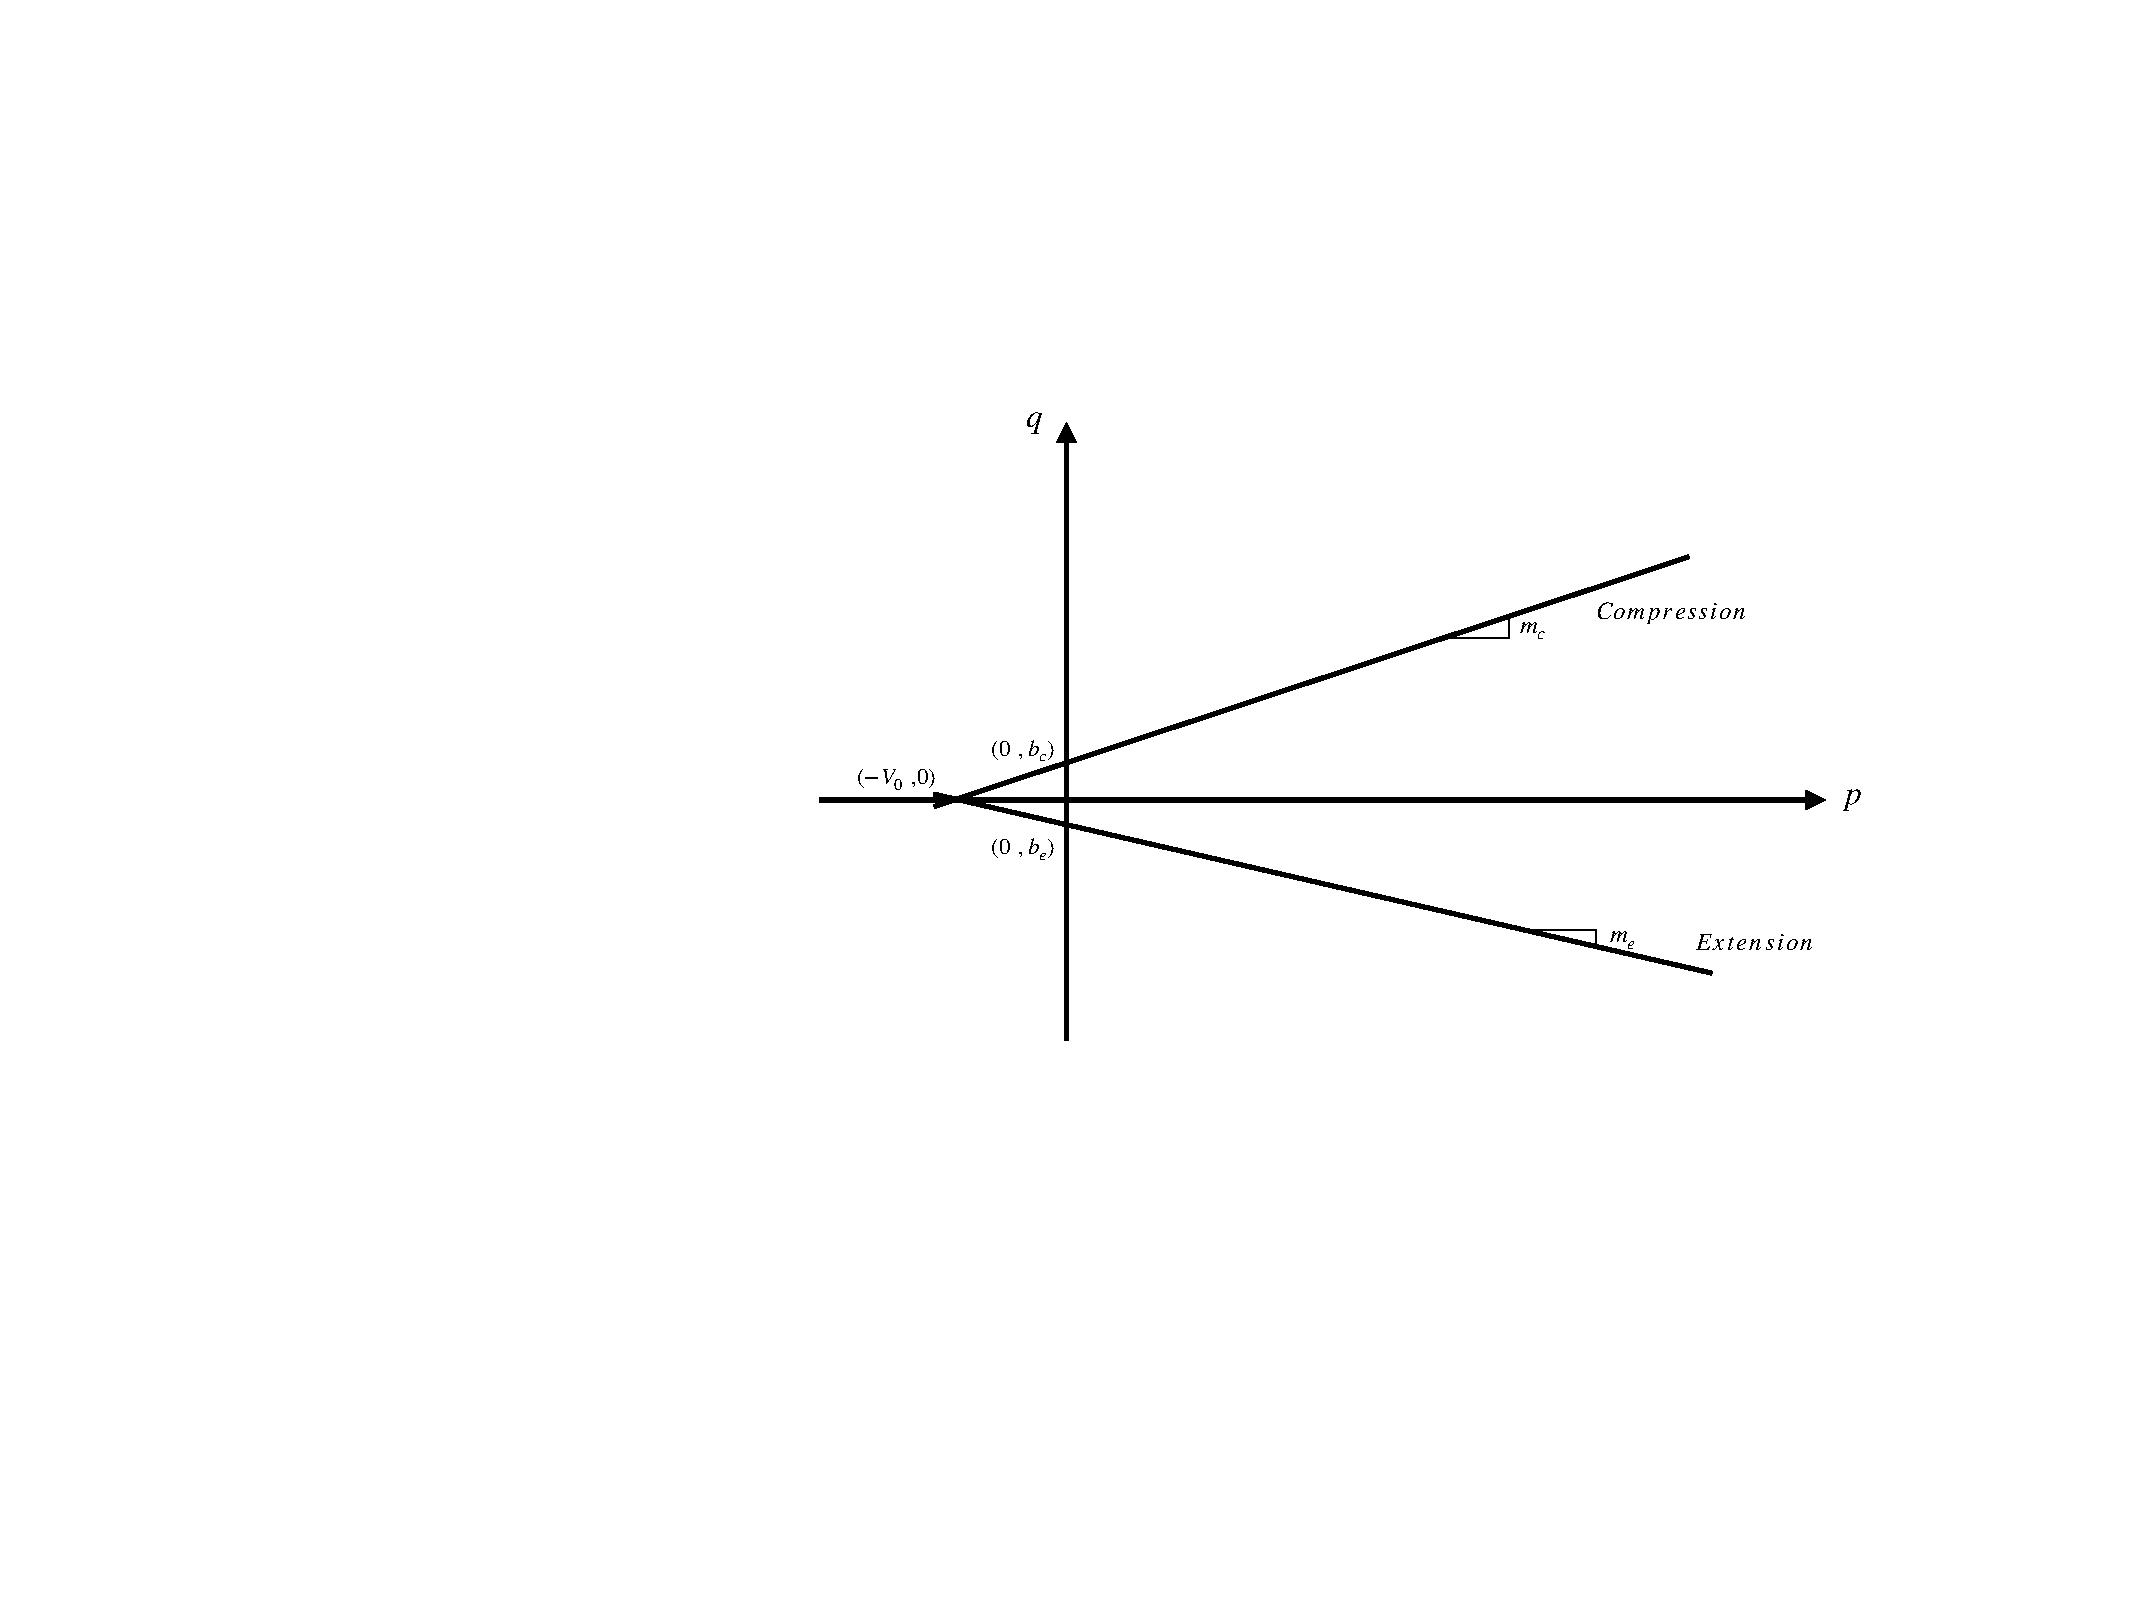
\includegraphics[width=\columnwidth]{ch5/mc_pq}
    \caption{Mohr-Coulomb criterion failure surface in  $(p-q)$ plane}
    \label{fig5:mc_pq}
\end{figure} 

Finally, the Mohr-Coulomb criterion is presented in the $\pi$-plane, obtained following the procedure described in section \ref{ch2:MC_pi} (cf. Figure \ref{fig5:mc_pi_plane}). 

\begin{figure}[tb]
    \centering
    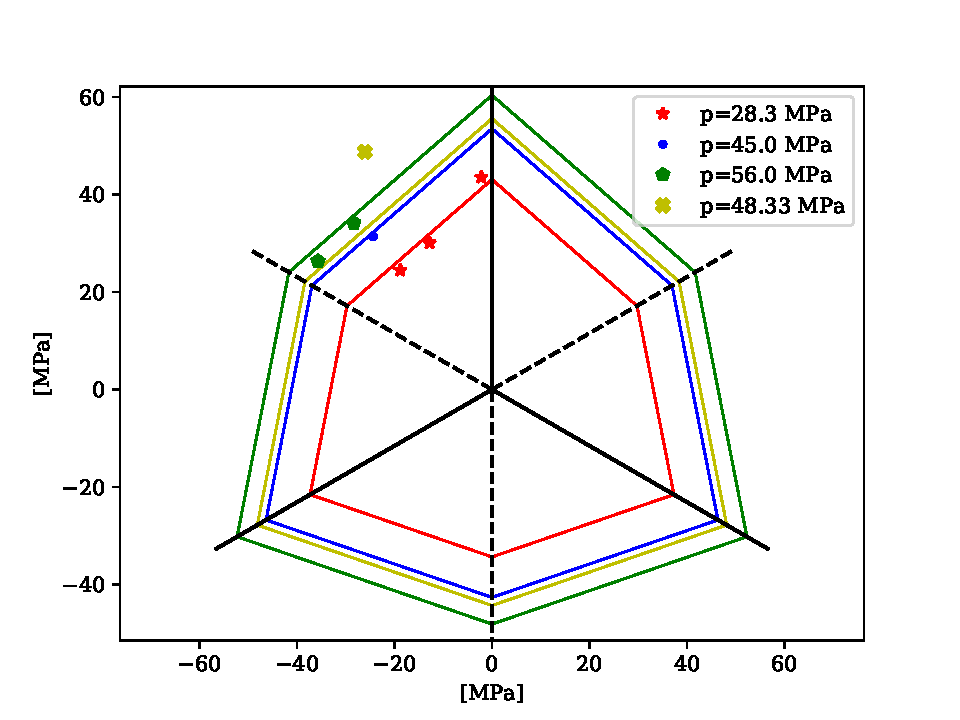
\includegraphics[width=0.7\columnwidth]{ch5/mc_pi_plane1}
    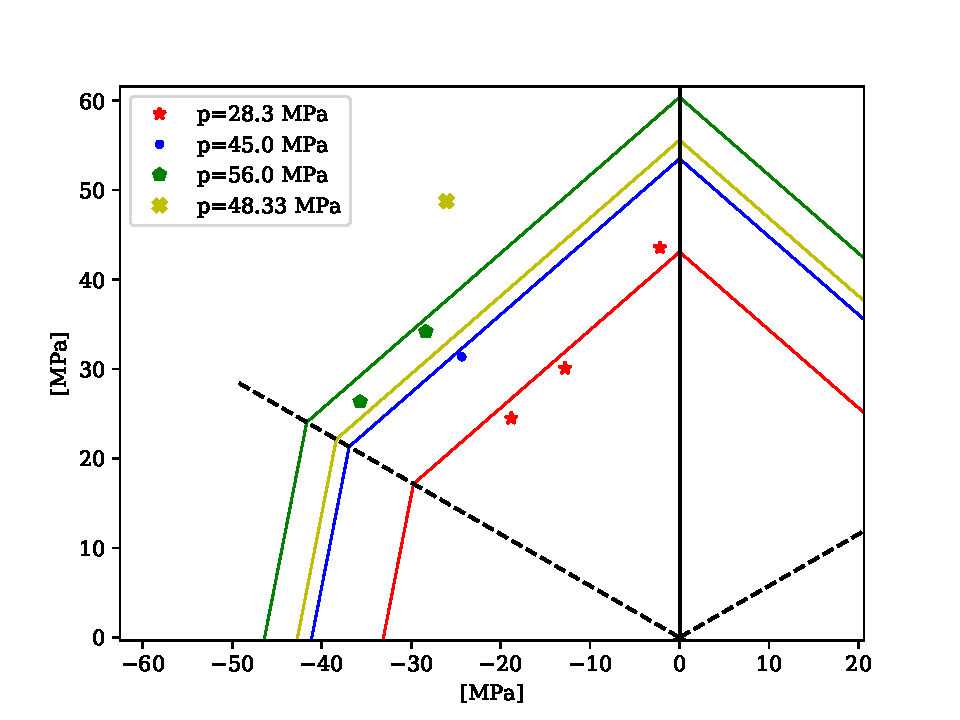
\includegraphics[width=0.7\columnwidth]{ch5/mc_pi_plane2}
    \caption{Mohr-Coulomb criterion failure surface in  $pi$- plane}
    \label{fig5:mc_pi_plane}
\end{figure} 



\subsection{Hoek-Brown failure criterion}
\subsection{Paul-Mohr-Coulomb failure criterion}
\section{Bi-linear Paul-Mohr-Coulomb failure criterion}\label{ch5:PMC}

Published data from rock testing in conventional triaxial and multi axial testing showed that the failure envelop is non-linear. This non-linearity can be approximated by fitting the experiments data using two planes instead of one, resulting in six parameters describing the envelop. 

The six-parameters fitting splits the data points in two sets in order to create two planes. These planes will give a better approximation of the failure envelop. The fitting procedure presented in 4.3.1. should then be applied to the two set of data points, resulting in different values of $\phi_c$,$\phi_e$ and $V_0$ for each plane.  

\section{Discussion}